% Reset counters and commands for appendix
\setcounter{chapter}{0}
\renewcommand{\thechapter}{\Alph{chapter}}
\setcounter{equation}{0}
\renewcommand{\theequation}{\Alph{chapter}.\arabic{equation}}
\setcounter{figure}{0}
\renewcommand{\thefigure}{\Alph{chapter}.\arabic{figure}}
\setcounter{table}{0}
\renewcommand{\thetable}{\Alph{chapter}.\arabic{table}}
\appendix
\chapter{Macでの研究環境の構築}
ここでは、Macで研究環境を構築する祭に最低限やるべきこと、知っておくべきことを説明します。Macに限らずWindowsやLinuxでも、計算機環境の設定は個々人の好みや研究内容によって大きく変わります。そのため、ここに書くことは参考程度にとどめて下さい。
\section{英語環境にする}
日本の研究室でMacを使う場合、OSの言語環境を日本語にしている人が多いでしょう。しかしMacを研究で使う場合には英語環境に変更することを強くお勧めします。大きく四つの理由があるからです。

まず第一に、インターネット上のMac関係の情報の多くが英語で書かれており、英語で検索した場合に見つかる情報の量と質は日本語の情報を圧倒するからです。使っているMacで何か問題が生じた場合にエラーメッセージが日本語で表示されていると、それを検索語にしても辿り着ける情報には限りがあります\footnote{\LaTeX 関係などの情報だと日本語特有の問題も発生しうるので、そこは臨機応変に対応して下さい。}。Apple社はアメリカの企業でありMacユーザの多くが北米に集中しています。そのためMac関連の情報のやり取りの多くは英語でなされています。これはMacに限らずコンピュータ関係全般に言えます\footnote{恐らく唯一の例外がRubyというプログラミング言語です。これは日本人により開発されたものが世界に広がった希有な例です。}

第二に、あなたは日本人のみと共同研究をするわけではないからです。もしあなたのMacの画面を外国人が見ながら、もしくはあなたが外国人のMacの画面を見ながら作業する時に、OSが英語環境になっていたほうが意志疎通が簡単になることは言うまでもないでしょう。また海外(特にアメリカ)の研究機関などで実験をするときに、現地で使用するMacが英語環境になっているのは当然です。

第三の理由は、ファイル名やメニューの表示が英語になっているほうが作業効率が上がるからです。Macだとホームディレクトリに「書類」や「デスクトップ」というディレクトリが存在しますが、英語環境ではそれぞれ「Documents」と「Desktop」です。Terminal.appからホームで\texttt{ls}すれば、実体が英語名だということがわかります。Finder.appからディレクトリの移動をしたいときに、英語環境であればホームを開いた状態で「do」と連打すれば「Documents」が選択された状態になります。また「de」と打てば「Desktop」が選択されます。日本語環境の場合にはこのようにはいきません。またメニューの「編集」は英語環境では「Edit」になっています。メニューで「Edit」を開いた状態で「co」と連打すれば「Copy」のところが選択された状態になるでしょう。

最後の理由は、できる限り英語に慣れ親しんだほうが良いからです。大学院に入りたての頃は、誰しも英語の読み書きと会話に苦労するでしょう。また日本人の多くの研究者はその後何十年も英語で苦労をし続けます。少しでも英語に慣れるため、常用するMacくらい英語環境で使う意志を持ちましょう。

ただし、英語環境にすることで問題が生じる場合があります。例えば英語環境でFLASHを表示すると日本語が文字化けすることがあります。これはFLASHが既に廃れつつある技術であり、かつFLASHの開発チームが能力不足だからです。他にも英語環境にすると日本語表示がうまくいかないソフトがあるかもしれませんが、そのようなソフトを使うのはやめましょう。日本語表示以外にも色々と問題を抱えている可能性があります。

図\ref{fig_English1_png}から図\ref{fig_English3_png}のように「システム環境設定」から英語環境に変更することができます。この設定後に起動したアプリケーションは、全て英語環境として起動されます。全てのメニューなどが英語で表示されるはずです。図\ref{fig_English3_png}にある「単語区切り」の設定は忘れないようにして下さい。ダブルクリックで日本語文字列を選択する場合に、熟語やカタカナ語が一つの単語として認識されるようになります。

\begin{figure}
  \begin{center}
    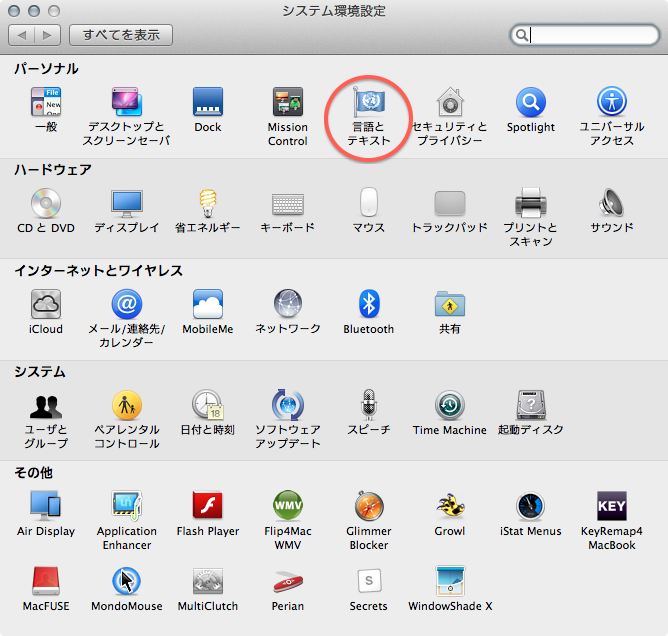
\includegraphics[scale=0.4,bb= 0 0 668 636]{fig/English1.png}
    \caption{「システム環境設定」から「言語とテキスト」を開く}
    \label{fig_English1_png}
  \end{center}
\end{figure}

\begin{figure}
  \begin{center}
    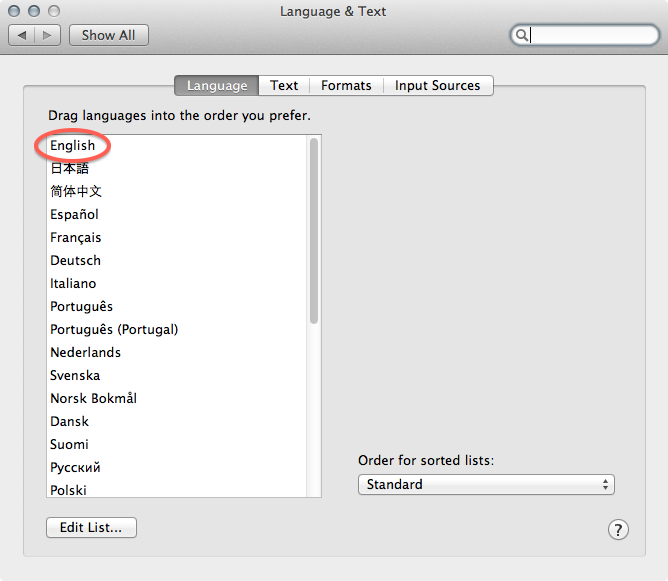
\includegraphics[scale=0.4,bb= 0 0 668 636]{fig/English2.png}
    \caption{「日本語」ではなく「English」を先頭に持ってくる(この画面は既に英語環境になっている場合のもの)}
    \label{fig_English2_png}
  \end{center}
\end{figure}

\begin{figure}
  \begin{center}
    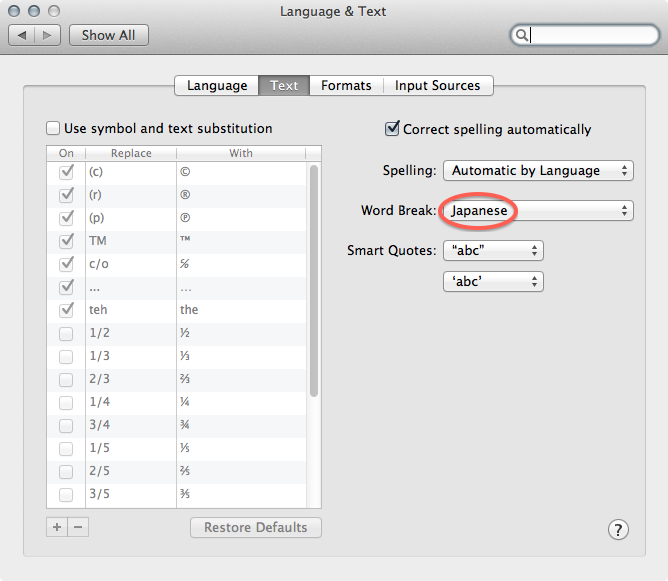
\includegraphics[scale=0.4,bb= 0 0 668 636]{fig/English3.png}
    \caption{「単語区切り(Word Break)」を「Japanese」にする(この画面は既に英語環境になっている場合のもの)}
    \label{fig_English3_png}
  \end{center}
\end{figure}


\section{拡張子を表示する}
Macの初期設定では、ファイルの拡張子(extension)が表示されません。図~\ref{fig_Extension_png}のようにFinder.appの「Preferences\ldots」から表示する設定に変更しましょう。この表示をしないと、Terminal.appから操作するファイル名とFinder.appからファイル名が見かけ上一致しない場合があります。

\begin{figure}
  \begin{center}
    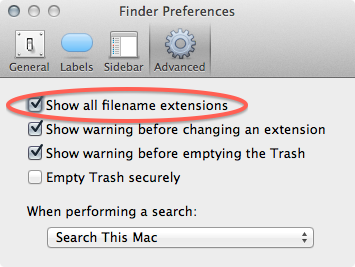
\includegraphics[scale=0.4,bb= 0 0 355 267]{fig/Extension.png}
    \caption{``Show all filename extensions''にチェックを入れると、全てのファイルで拡張子が表示されるようになる}
    \label{fig_Extension_png}
  \end{center}
\end{figure}

\section{キーボードの設定}

\subsection{Caps LockキーをControlキーに変更する}
もしあなたのMacがUS配列のキーボードならば、Caps LockキーはControlキーとして機能するように設定を変更しましょう。図\ref{fig_Keyboard1_png}のように、System Preferencesから「Keyboard」を開いて「Keyboard」タブの「Modifier keys\ldots」を押し、Caps LockをControlにします。後述するように、OS~X環境ではEmacsの操作体系に倣ったキーボードショートカットが使われています。そのため、Controlキーの使用率が他のOSに比べて非常に高くなるのが特徴です。US配列のキーボードを使用している場合にはControlキーが押しにくい位置にあるため、滅多に使わない、かつ最も押しやすい位置にあるCaps LockをControlキーにしてしまうことがよく行われています。

\begin{figure}
  \begin{center}
    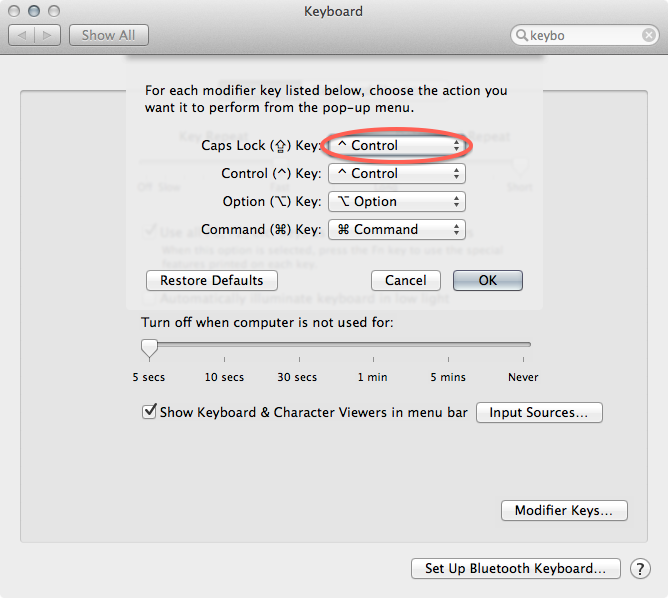
\includegraphics[scale=0.4,bb= 0 0 668 636]{fig/Keyboard1.png}
    \caption{Caps LockをControlキーに変更する}
    \label{fig_Keyboard1_png}
  \end{center}
\end{figure}

\subsection{Tabキーの動作の変更}
次に、図\ref{fig_Keyboard2_png}のように「Keyboard Shortcuts」のタブに移動し、ボタンなどの選択を全てTabキーで行えるようにします。このようにすることで、様々な画面操作をするときに、いちいちキーボードからトラックパッドやマウスへ手の移動をしなくて済むようになります。

\begin{figure}
  \begin{center}
    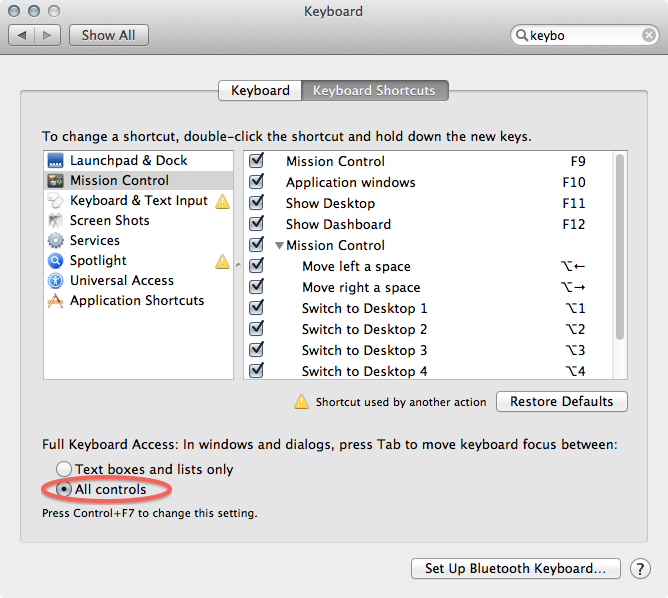
\includegraphics[scale=0.4,bb= 0 0 668 636]{fig/Keyboard2.png}
    \caption{全てのボタンなどをtabキーで移動できるようにする}
    \label{fig_Keyboard2_png}
  \end{center}
\end{figure}

例えば、Mac の電源ボタンを軽く一度だけ押すと、図\ref{fig_reboot_png}のような確認ダイアログが出てくるはずです。ここで数回Tabキーを押すと、「Cancel」ボタンが強調表示されるようになります。また「Shut Down」ボタンが明滅しているでしょう。この状態でSpaceキーを押すと、マウスやトラックパッドの操作をしなくても強調表示された「Cancel」ボタンが押されます。またReturnキーを押すと明滅している「Shut Down」ボタンがおされてMacが再起動します。このように、Macではダイアログのボタンをクリックする代わりにSpaceキーとReturnキーで操作することができます。

\begin{figure}
  \begin{center}
    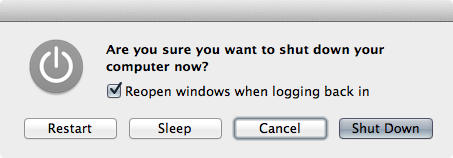
\includegraphics[scale=0.4,bb= 0 0 453 158]{fig/reboot.png}
    \caption{再起動の確認ダイアログ。Tabを数回押すと、「Cancel」が強調表示される。「Shut Down」は明滅している。}
    \label{fig_reboot_png}
  \end{center}
\end{figure}

\subsection{Spotlightのショートカットの変更}
最後に、Spotlightのショートカットを図\ref{fig_Keyboard3_png}のようにControl-Space(画面上の表示は「\verb|^|Space」)の組み合わせからCommand-Space(画面上の表示は「\UTF{2318}Space」)などの組み合わせに変更しましょう。Control-Spaceは後述するようにEmacsで頻繁に使用するショートカットであるため、Spotlightのショートカットとして使用されてしまうと不便だからです。

\begin{figure}
  \begin{center}
    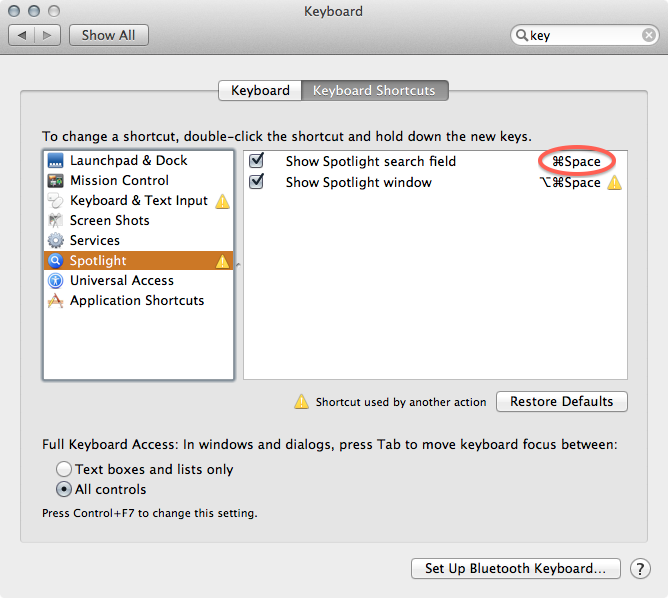
\includegraphics[scale=0.4,bb= 0 0 668 636]{fig/Keyboard3.png}
    \caption{Spotlightのショートカットを「Control-Space」から「Command-Space」に変更した状態}
    \label{fig_Keyboard3_png}
  \end{center}
\end{figure}

\section{KeyRemap4MacBook}

\section{zsh}
\section{MacPorts}
\subsection{Emacs}
\subsection{\LaTeX}

\section{Emacsの操作体系に慣れる}

\begin{table}
\begin{center}
\caption{}
\label{tab_emacs}
\begin{tabular}{lll}
\hline
ショートカット & 英単語 & 機能 \\ \hline\hline
C-f & {\bf F}orward & 一文字進む(→キーと同等) \\
C-b & {\bf B}ackward & 一文字戻る(←キーと同等) \\
C-p & {\bf P}revious line & 次の行へ進む(↓キーと同等) \\
C-n & {\bf N}ext line & 前の行へ戻る(↑キーと同等) \\
C-a & {\bf A}head & 行頭へ移動 \\
C-e & {\bf E}nd & 行末へ移動 \\
C-k & {\bf K}ill & カーソル位置から行末までを全てバッファに移動(カットに類似) \\
C-y & {\bf Y}ank & バッファにあるものをカーソル位置にペースト \\
C-t & {\bf T}ranspose & カーソルの前後の文字を入れ替える \\
C-h & 不明 & カーソル前方を一文字削除(MacのDelete、WindowsのBackspaceと同等) \\
C-d & forward {\bf D}elete & カーソル後方を一文字削除(WindowsのDeleteと同等) \\
C-m & 不明 & 改行(カーソルも次の行へ移動する) \\
C-o & 不明 line & 改行(カーソルは元の位置にとどまる) \\ \hline
\end{tabular}
\end{center}
\end{table}


\section{Xcode}